\chapter{Grounding Surgical Action Triplets with Instrument Instance Segmentation}
\chaptermark{Triplet Grounding}
\label{chap:triplet-grounding}
\minitoc

\newcommand{\ivt}{\texttt{<instrument, verb, target>}\xspace}
\newcommand{\triplet}[3]{\texttt{<#1, #2, #3>}\xspace}
\newcommand{\tripmap}{\ensuremath{\mathrm{mAP}}\xspace}

\begin{center}
\begin{minipage}[b]{0.9\linewidth}
\small
\textbf{Chapter note.}
This chapter adapts material from the manuscript \emph{Grounding Surgical Action Triplets with Instrument Instance Segmentation: A Dataset and Target-Aware Fusion Approach}. It builds directly on CholecInstanceSeg by using instrument instance masks as the spatial support for surgical action triplets.
\end{minipage}
\end{center}

\section{Overview}
\label{sec:triplet-grounding-overview}

The previous chapter established CholecInstanceSeg as a dataset for distinguishing and segmenting individual surgical instruments. This chapter asks the next question: once an instrument instance has been localised, can its action and anatomical target be predicted in a spatially grounded way?

Surgical action triplets represent instrument-tissue interactions as \ivt tuples. For example, \triplet{Grasper}{Grasp}{Gallbladder} and \triplet{Hook}{Dissect}{Gallbladder} describe not only which instrument is present, but also what it is doing and which anatomical structure is involved. This representation is useful because surgical progress and safety are defined by interactions rather than by isolated objects. However, most existing triplet-recognition methods operate at the frame level: they predict which triplets occur somewhere in the image without identifying the instrument instance responsible for each action.

This chapter introduces triplet segmentation, a task that unifies instrument instance segmentation with surgical action triplet prediction. A triplet segmentation model outputs pixel-level instrument masks, and each mask is assigned an instrument, verb, and target label. This makes the prediction spatially grounded and interpretable: each predicted interaction is tied to a visible instrument instance.

\begin{figure}[ht]
\centering
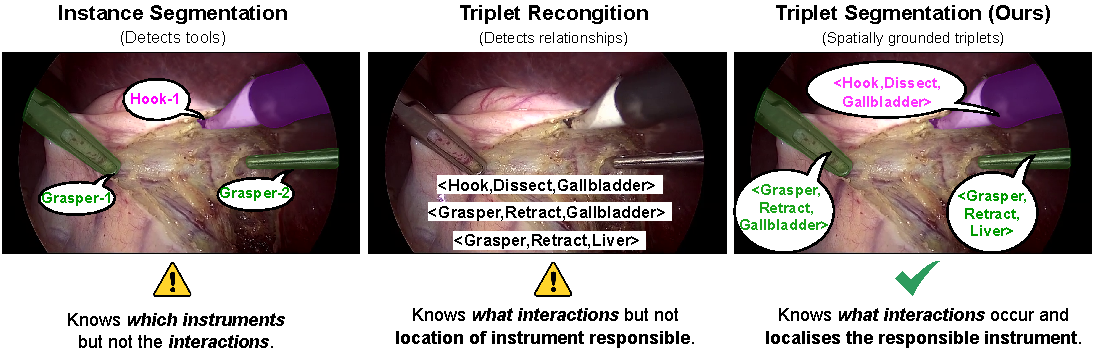
\includegraphics[width=\linewidth]{figs/triplet_grounding/instance_recognition_triplet_segmentation.pdf}
\caption{Comparison of instance segmentation, frame-level triplet recognition, and triplet segmentation. Triplet segmentation grounds each \ivt prediction to an instrument instance mask, making the interaction spatially interpretable.}
\label{fig:triplet-grounding-task}
\end{figure}

The chapter makes four contributions. First, it defines triplet segmentation as a spatially grounded surgical action understanding task. Second, it presents CholecTriplet-Seg, a dataset that links CholecInstanceSeg instrument masks with CholecT50 action triplets. Third, it introduces a triplet segmentation evaluation protocol based on recognition, detection, and segmentation mAP. Fourth, it presents TargetFusionNet, a target-aware model that uses weak anatomical priors to improve triplet prediction.

\section{From Frame-Level Triplets to Instance-Level Grounding}
\label{sec:triplet-grounding-from-frame}

Triplet recognition was introduced to model fine-grained instrument-tissue interactions in laparoscopic video \cite{1nywoye_rec_action_triplets,NWOYE2022102433_rendevous}. In this formulation, an image may contain multiple valid triplets, and the model predicts which triplets are present. While this is a powerful representation, frame-level recognition has a structural limitation: it does not indicate which instrument performs which action.

This limitation becomes important in multi-instrument scenes. If two graspers are visible and the frame-level labels include \triplet{Grasper}{Retract}{Liver} and \triplet{Grasper}{Grasp}{Gallbladder}, the labels alone do not say which grasper corresponds to which interaction. A model can therefore achieve a correct frame-level prediction while still failing to provide a clinically or visually meaningful explanation of the scene.

Earlier spatial grounding approaches relied primarily on class activation maps or bounding boxes, which provide coarse localisation but do not explicitly link actions to precise instrument instances. This is particularly limiting for laparoscopic tools, which are elongated, thin, often non-axis-aligned, and frequently overlap tissue or other instruments. Pixel-level instance masks are a more suitable spatial representation.

Triplet segmentation addresses this by requiring each predicted triplet to be associated with an instrument instance mask. Given an input image \(x \in \mathbb{R}^{H \times W \times 3}\), the model predicts a set of masks \(M = \{M_k\}\), where each mask is associated with a triplet:

\[
    \mathcal{T} = \{ \langle I_k, v_k, t_k \rangle \mid M_k \in M \}.
\]

Here \(I_k\), \(v_k\), and \(t_k\) denote the instrument, verb, and target for instance \(k\). The task therefore evaluates both whether the interaction is classified correctly and whether it is localised to the correct instrument instance.

\section{CholecTriplet-Seg}
\label{sec:triplet-grounding-dataset}

CholecTriplet-Seg was constructed by aligning frame-level triplet annotations from CholecT50 \cite{NWOYE2022102433_rendevous} with instrument instance masks from CholecInstanceSeg \cite{cholecinstanceseg}. The resulting dataset contains 30,955 frames from 50 laparoscopic cholecystectomy videos, with 49,866 spatially grounded triplets.

\begin{table}[ht]
\centering
\begin{tabular}{l|c|l|c}
\hline
\textbf{Dataset} & \textbf{Videos} & \textbf{Annotation type} & \textbf{Frames} \\
\hline
CholecT50 \cite{NWOYE2022102433_rendevous} & 50 & Frame-level triplet labels & 100,861 \\
CholecInstanceSeg \cite{cholecinstanceseg} & 85 & Instrument instance masks & 41,933 \\
CholecTriplet-Seg & 50 & Triplet + instance masks & 30,955 \\
\hline
\end{tabular}
\caption{Datasets involved in constructing CholecTriplet-Seg. CholecTriplet-Seg combines the semantic interaction labels of CholecT50 with the spatial instance masks of CholecInstanceSeg.}
\label{tab:triplet-grounding-source-datasets}
\end{table}

The triplet vocabulary follows CholecT50: six instruments, ten verbs, and fifteen anatomical targets. Although these categories produce 900 possible instrument-verb-target combinations, CholecT50 restricts the vocabulary to 100 clinically meaningful triplets. CholecTriplet-Seg adopts this clinically informed vocabulary for comparability with previous work; 93 of the 100 valid triplets appear in the final aligned dataset.

\subsection{Alignment and Annotation Format}
\label{sec:triplet-grounding-alignment}

The annotation schema extends the LabelMe-style structure used by CholecInstanceSeg. Each instrument shape already contains a class label, polygon points, and an instance group identifier. CholecTriplet-Seg adds two fields: the verb and the anatomical target. If an instrument instance is represented by multiple polygons, all polygons share the same group identifier, label, verb, and target.

The initial alignment matched CholecT50 triplets to CholecInstanceSeg masks using frame correspondence and instrument class. This automatic process was insufficient in several common cases because CholecT50 labels are frame-level rather than instance-level. Manual verification and correction were therefore required to ensure that each triplet was assigned to the correct instrument mask.

Two types of inconsistencies were especially important:

\begin{itemize}
\item \textbf{Matching errors}: frames where multiple instruments of the same class were associated with different actions, making automatic assignment ambiguous. These affected 2,361 frames.
\item \textbf{Conflict errors}: frames where the segmentation and triplet annotations disagreed, such as missing masks, redundant triplets, or mismatched class labels. These affected 7,194 frames.
\end{itemize}

\begin{figure}[ht]
\centering
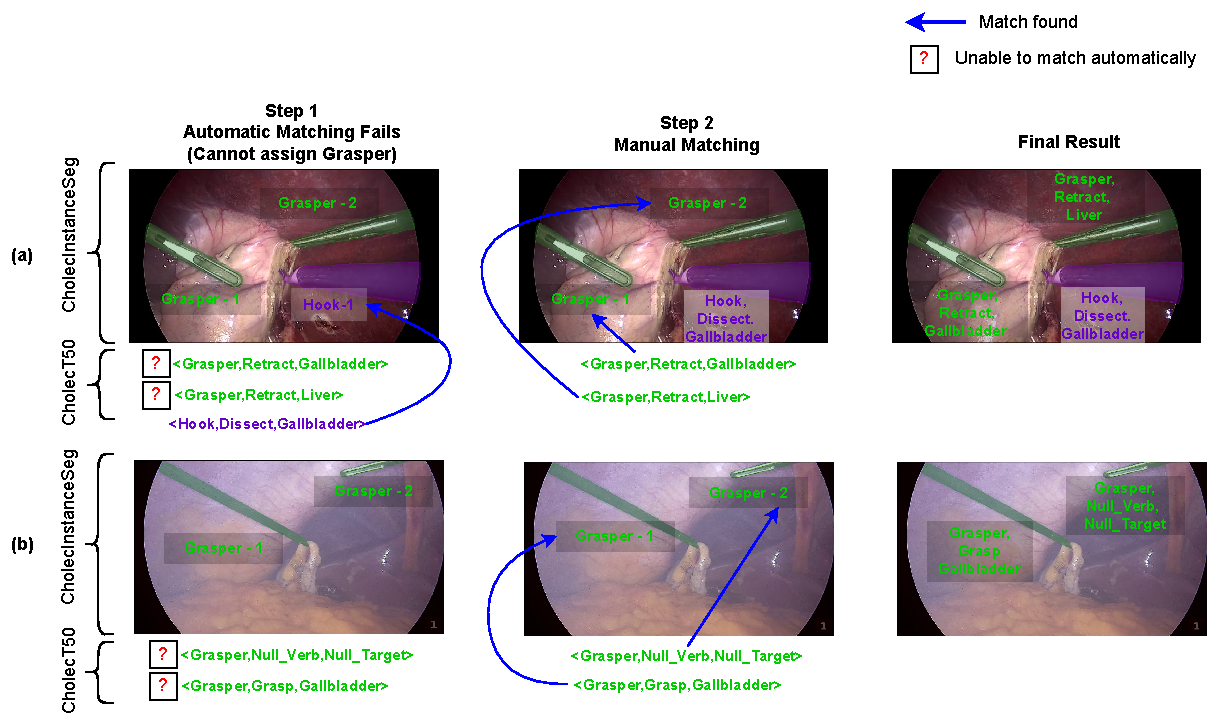
\includegraphics[width=\linewidth]{figs/triplet_grounding/matching_errors.pdf}
\caption{Examples of matching errors. Multiple instruments of the same class can perform different actions, so frame-level triplets must be manually linked to the correct instrument instance.}
\label{fig:triplet-grounding-matching-errors}
\end{figure}

\begin{figure}[ht]
\centering
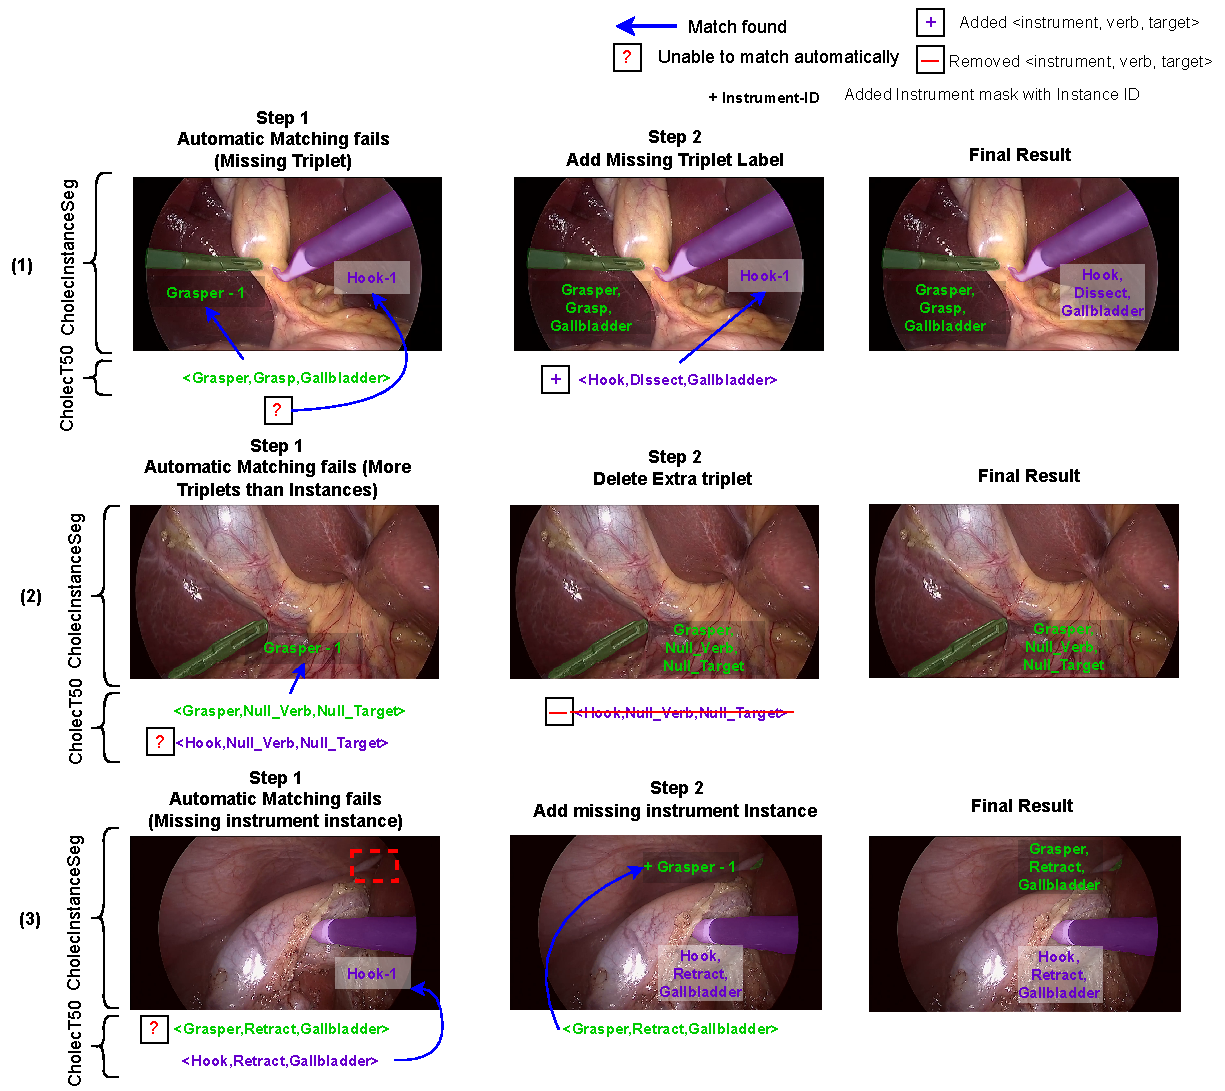
\includegraphics[width=\linewidth]{figs/triplet_grounding/conflict_errors.pdf}
\caption{Examples of conflict errors between source annotations, including missing triplets, redundant triplets, and missing instrument masks.}
\label{fig:triplet-grounding-conflict-errors}
\end{figure}

After alignment, a full dataset pass was performed to enforce schema consistency and verify that each instrument instance had a verb and target assignment. This process produced a strongly supervised benchmark for instance-level triplet grounding.

\subsection{Splits and Class Imbalance}
\label{sec:triplet-grounding-splits}

CholecTriplet-Seg follows the CholecInstanceSeg split protocol to avoid leakage between training and evaluation data. The dataset contains 45 training videos, one validation video, and four test videos. The split statistics are shown in \tabref{tab:triplet-grounding-split-stats}.

\begin{table}[ht]
\centering
\begin{tabular}{l|c|c|c|c}
\hline
\textbf{Split} & \textbf{Videos} & \textbf{Images} & \textbf{Triplets} & \textbf{Avg. triplets/frame} \\
\hline
Train & 45 & 22,818 & 37,591 & 1.65 \\
Validation & 1 & 2,496 & 3,341 & 1.34 \\
Test & 4 & 5,641 & 8,934 & 1.58 \\
\hline
Total & 50 & 30,955 & 49,866 & 1.61 \\
\hline
\end{tabular}
\caption{CholecTriplet-Seg split statistics.}
\label{tab:triplet-grounding-split-stats}
\end{table}

Like many surgical datasets, CholecTriplet-Seg is long-tailed. A small number of common triplets dominate the dataset, while many clinically valid triplets occur rarely. This imbalance is visible both at the full triplet level and within the individual instrument, verb, and target categories.

\begin{figure}[ht]
\centering
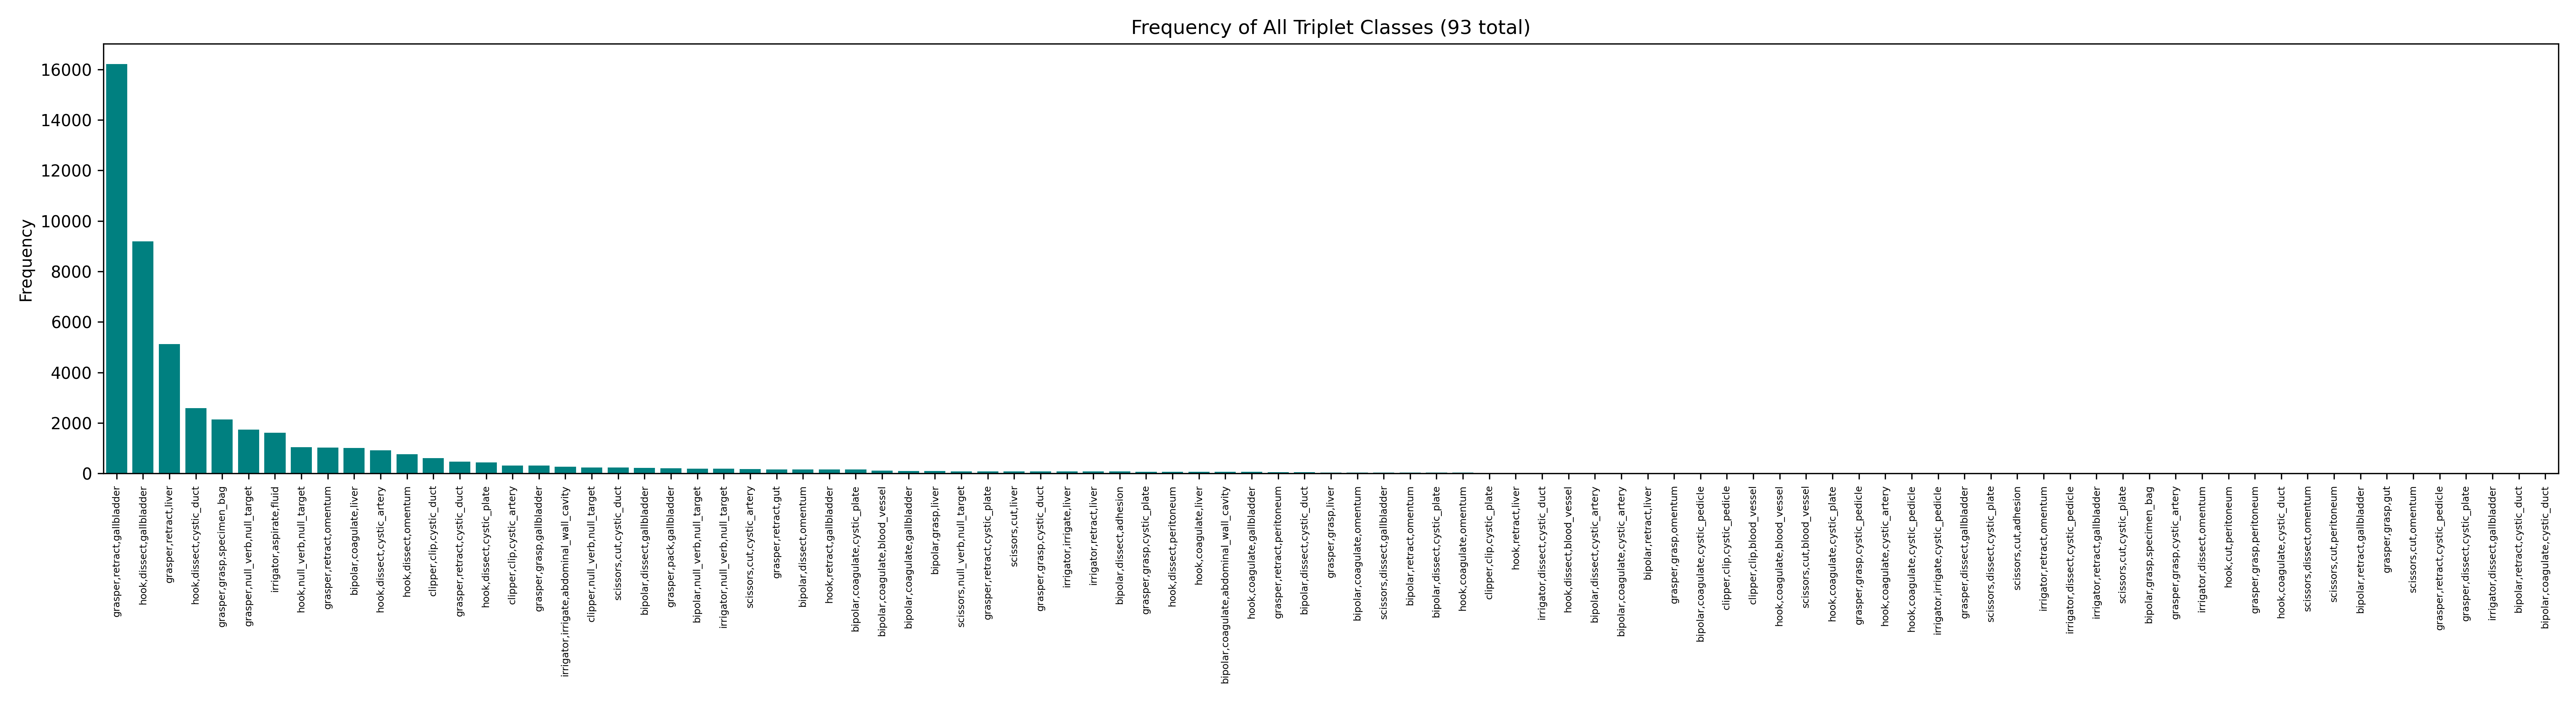
\includegraphics[width=\linewidth]{figs/triplet_grounding/all_triplets_frequency.png}
\caption{Frequency distribution of triplet classes in CholecTriplet-Seg. The dataset has a long-tailed distribution, with a small number of frequent triplets and many rare triplets.}
\label{fig:triplet-grounding-triplet-frequency}
\end{figure}

\section{Evaluation Protocol}
\label{sec:triplet-grounding-metric}

Triplet segmentation requires evaluation of both semantic correctness and spatial grounding. This chapter therefore reports three related evaluation modes.

\begin{description}
\item[Recognition mAP] evaluates whether triplets are present in a frame, regardless of spatial alignment. This corresponds to the standard frame-level classification setting used in CholecT50.
\item[Detection mAP] evaluates whether each predicted triplet is correctly associated with an instrument bounding box, using bounding-box IoU for localisation.
\item[Segmentation mAP] evaluates whether each predicted triplet is correctly associated with an instrument instance mask, using mask IoU for pixel-level grounding.
\end{description}

Metrics are reported for individual components (\(\tripmap_I\), \(\tripmap_V\), \(\tripmap_T\)), component pairs (\(\tripmap_{IV}\), \(\tripmap_{IT}\)), and full triplets (\(\tripmap_{IVT}\)). Superscripts indicate the evaluation mode, such as \(\tripmap_{IVT}^{seg}\) for full triplet segmentation mAP. The full triplet score is the strictest measure because a prediction must correctly identify the instrument, verb, target, and spatial support.

\section{TargetFusionNet}
\label{sec:triplet-grounding-method}

The main modelling challenge in triplet segmentation is target prediction. Instrument classes are visually distinctive and are directly tied to the mask. Verbs can often be inferred from tool pose and local motion cues, although this chapter uses single frames. Anatomical targets are harder: they may have weak boundaries, similar appearance, partial visibility, and ambiguous definitions. Pixel-level target annotations for the CholecTriplet-Seg target vocabulary are unavailable, and producing them would require extensive expert labelling.

TargetFusionNet addresses this bottleneck by incorporating weak anatomical priors into an instance segmentation architecture. The model builds on Mask2Former \cite{cheng2022masked}, using transformer queries to predict masks and labels. It augments the decoder with a target-aware fusion mechanism that injects coarse anatomical information derived from EndoViT \cite{batic2024endovit}, a tissue segmentation model trained on CholecSeg8k \cite{cholecseg8k}.

\begin{figure}[ht]
\centering
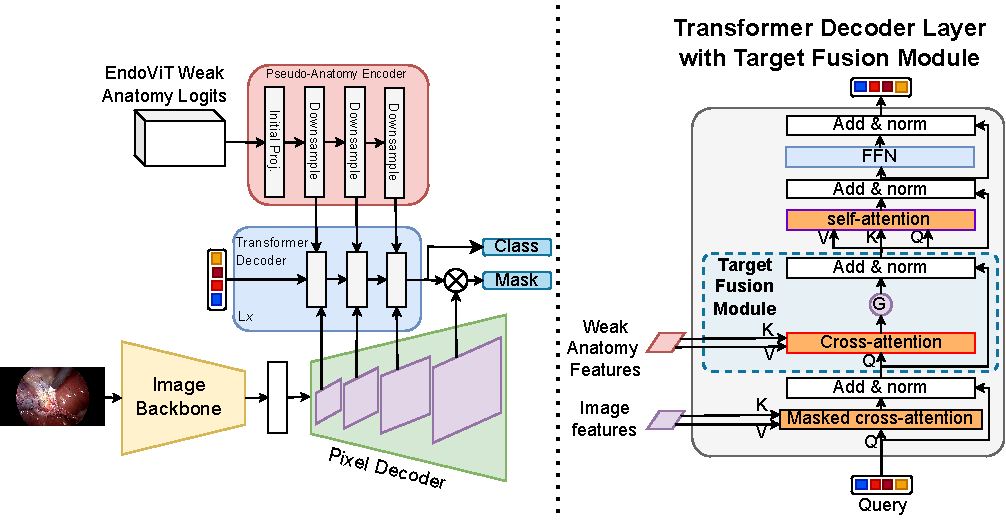
\includegraphics[width=\linewidth]{figs/triplet_grounding/target_fusion.pdf}
\caption{Overview of TargetFusionNet. Weak anatomical logits are encoded into multi-scale target-prior features and fused with Mask2Former decoder queries through gated cross-attention.}
\label{fig:triplet-grounding-targetfusionnet}
\end{figure}

The anatomical priors are weak rather than definitive. EndoViT predicts broad tissue categories that only partially align with the CholecTriplet-Seg target vocabulary. For example, some outputs correspond closely to surgical targets, while others are approximate or cover multiple target categories. TargetFusionNet therefore treats these logits as noisy spatial context rather than as ground truth.

The target fusion mechanism has three parts:

\begin{itemize}
\item \textbf{Weak-anatomy encoder}: EndoViT logits are projected into the decoder feature dimension and downsampled into multi-scale feature maps.
\item \textbf{Target-aware decoder}: Mask2Former decoder layers are augmented so that instance queries can attend to the weak-anatomy features.
\item \textbf{Gated cross-attention}: a learned gate controls how much anatomical context is injected into each query.
\end{itemize}

For a query \(Q\) and weak-anatomy key/value features \((K_t,V_t)\), the gated update is:

\[
Q' = Q + \sigma(W_g A) \odot A,
\qquad
A = \mathrm{Attn}(Q, K_t, V_t),
\]

where \(A\) is the cross-attention output, \(W_g\) is a learnable linear layer, \(\sigma\) is the sigmoid function, and \(\odot\) denotes element-wise multiplication. The gate allows the network to use anatomical priors when they are helpful while suppressing them when they are noisy or misleading.

Each predicted instance mask receives a single label from the 100 clinically valid triplet classes. This 100-class formulation preserves triplet coherence: the network predicts a valid instrument-verb-target combination rather than three independent labels that may not form a meaningful triplet.

\section{Experiments}
\label{sec:triplet-grounding-experiments}

TargetFusionNet was evaluated against three baselines:

\begin{itemize}
\item \textbf{RDV-Det}: a weakly grounded baseline derived from the Rendezvous framework, using class activation maps for coarse localisation \cite{nwoye2023cholectriplet2022}.
\item \textbf{RDV + Mask2Former}: a hybrid baseline that replaces weak localisation with Mask2Former instance masks while retaining the RDV triplet association mechanism.
\item \textbf{Mask2Former-Triplet}: a strong instance-level baseline that extends Mask2Former with a 100-class triplet head but does not include the target-aware fusion module.
\end{itemize}

TargetFusionNet was implemented in MMDetection \cite{mmdetection} with a ResNet-50 \cite{resnet} backbone pretrained for instrument segmentation. Images were resized to \(1024 \times 1024\), and training used AdamW \cite{loshchilov2017decoupled} with random horizontal flipping, cropping, and scaling. Experiments were performed on a single NVIDIA A100 GPU, and the best checkpoint was selected using validation mask mAP.

\section{Results}
\label{sec:triplet-grounding-results}

\Tabref{tab:triplet-grounding-overall-results} reports performance across segmentation, detection, and recognition. The main metric is \(\tripmap_{IVT}^{seg}\), since it evaluates complete triplet correctness with instance-mask grounding.

\begin{table}[ht]
\centering
\resizebox{\linewidth}{!}{
\begin{tabular}{llcccccc}
\hline
\textbf{Evaluation} & \textbf{Method} & \(\tripmap_I\) & \(\tripmap_V\) & \(\tripmap_T\) & \(\tripmap_{IV}\) & \(\tripmap_{IT}\) & \(\tripmap_{IVT}\) \\
\hline
Segmentation & RDV-Det & 0.09 & 0.11 & 0.08 & 0.08 & 0.04 & 0.03 \\
Segmentation & RDV + Mask2Former & 48.11 & 32.51 & 16.29 & 14.40 & 11.38 & 8.73 \\
Segmentation & Mask2Former-Triplet & 65.24 & 45.61 & 20.75 & 23.03 & 16.47 & 12.23 \\
Segmentation & TargetFusionNet & \textbf{67.19} & \textbf{46.27} & \textbf{21.55} & \textbf{24.93} & \textbf{17.75} & \textbf{13.47} \\
\hline
Detection & RDV-Det & 3.28 & 2.86 & 0.29 & 1.43 & 0.77 & 0.55 \\
Detection & RDV + Mask2Former & 54.28 & 34.48 & 13.54 & 16.56 & 9.30 & 6.72 \\
Detection & Mask2Former-Triplet & 64.64 & 45.35 & 20.64 & 22.94 & 16.42 & 12.19 \\
Detection & TargetFusionNet & \textbf{66.52} & \textbf{46.23} & \textbf{23.70} & \textbf{24.82} & \textbf{17.74} & \textbf{13.45} \\
\hline
Recognition & RDV-Det & 80.55 & 61.44 & 40.83 & 35.93 & 34.47 & 27.17 \\
Recognition & RDV + Mask2Former & 80.55 & 61.44 & 40.83 & 35.93 & 34.47 & 27.17 \\
Recognition & Mask2Former-Triplet & 82.70 & 64.64 & 50.22 & 39.79 & 39.93 & 32.28 \\
Recognition & TargetFusionNet & \textbf{86.61} & \textbf{71.93} & \textbf{51.19} & \textbf{44.48} & \textbf{43.24} & \textbf{34.23} \\
\hline
\end{tabular}}
\caption{Triplet segmentation, detection, and recognition results. Values are mAP scores for instruments, verbs, targets, pairs, and full triplets.}
\label{tab:triplet-grounding-overall-results}
\end{table}

The results show three important trends. First, weak localisation is insufficient for instance-level triplet grounding: RDV-Det achieves only 0.03 \(\tripmap_{IVT}^{seg}\). Second, adding strong instance masks provides a large improvement, raising \(\tripmap_{IVT}^{seg}\) to 8.73 in RDV + Mask2Former. Third, jointly predicting masks and triplet labels with Mask2Former-Triplet improves the score to 12.23, while TargetFusionNet reaches 13.47 by incorporating target-aware fusion.

The detection and recognition results show the same pattern. TargetFusionNet achieves the best full-triplet detection score, \(\tripmap_{IVT}^{det}=13.45\), and the best recognition score, \(\tripmap_{IVT}^{rec}=34.23\). The recognition results are higher than the segmentation scores because they do not require spatial grounding; however, the segmentation scores are the more relevant measure for this chapter's goal.

\subsection{Fusion Ablations}
\label{sec:triplet-grounding-ablations}

\Tabref{tab:triplet-grounding-fusion-ablation} compares TargetFusionNet with early and late fusion variants. Early fusion concatenates weak anatomical logits with the RGB image before the backbone. Late fusion injects the logits after the decoder. TargetFusionNet performs mid-level gated fusion inside the transformer decoder.

\begin{table}[ht]
\centering
\resizebox{\linewidth}{!}{
\begin{tabular}{lcccccc}
\hline
\textbf{Method} & \(\tripmap_I^{seg}\) & \(\tripmap_V^{seg}\) & \(\tripmap_T^{seg}\) & \(\tripmap_{IV}^{seg}\) & \(\tripmap_{IT}^{seg}\) & \(\tripmap_{IVT}^{seg}\) \\
\hline
TargetFusionNet & 67.19 & 46.27 & \textbf{21.55} & 24.93 & \textbf{17.75} & \textbf{13.47} \\
Early-concat & \textbf{69.13} & \textbf{50.74} & 21.52 & \textbf{27.62} & 16.83 & 12.21 \\
Late-concat & 59.90 & 40.65 & 20.21 & 23.17 & 16.07 & 10.99 \\
\hline
\end{tabular}}
\caption{Segmentation mAP for target-fusion strategies. Although early fusion improves some component scores, TargetFusionNet gives the best full-triplet segmentation score.}
\label{tab:triplet-grounding-fusion-ablation}
\end{table}

Early fusion improves some component scores, especially instrument and verb segmentation, but does not improve full triplet segmentation. This suggests that better component predictions do not necessarily produce coherent instrument-verb-target combinations. Late fusion performs worse, indicating that anatomical context is less useful when injected only after the decoder has already formed its instance representations. The gated decoder-level fusion in TargetFusionNet offers the best full triplet performance.

\subsection{Qualitative Results}
\label{sec:triplet-grounding-qualitative}

\Figref{fig:triplet-grounding-qualitative} compares predictions from RDV-Det, RDV + Mask2Former, Mask2Former-Triplet, and TargetFusionNet. The examples show that all methods can perform reasonably in simple single-instrument cases, but differences emerge in complex frames containing multiple instruments, occlusion, or rare targets. TargetFusionNet more consistently links the correct instrument instance to the correct target, particularly in cases where weak anatomical priors help distinguish visually similar structures.

\begin{figure}[ht]
\centering
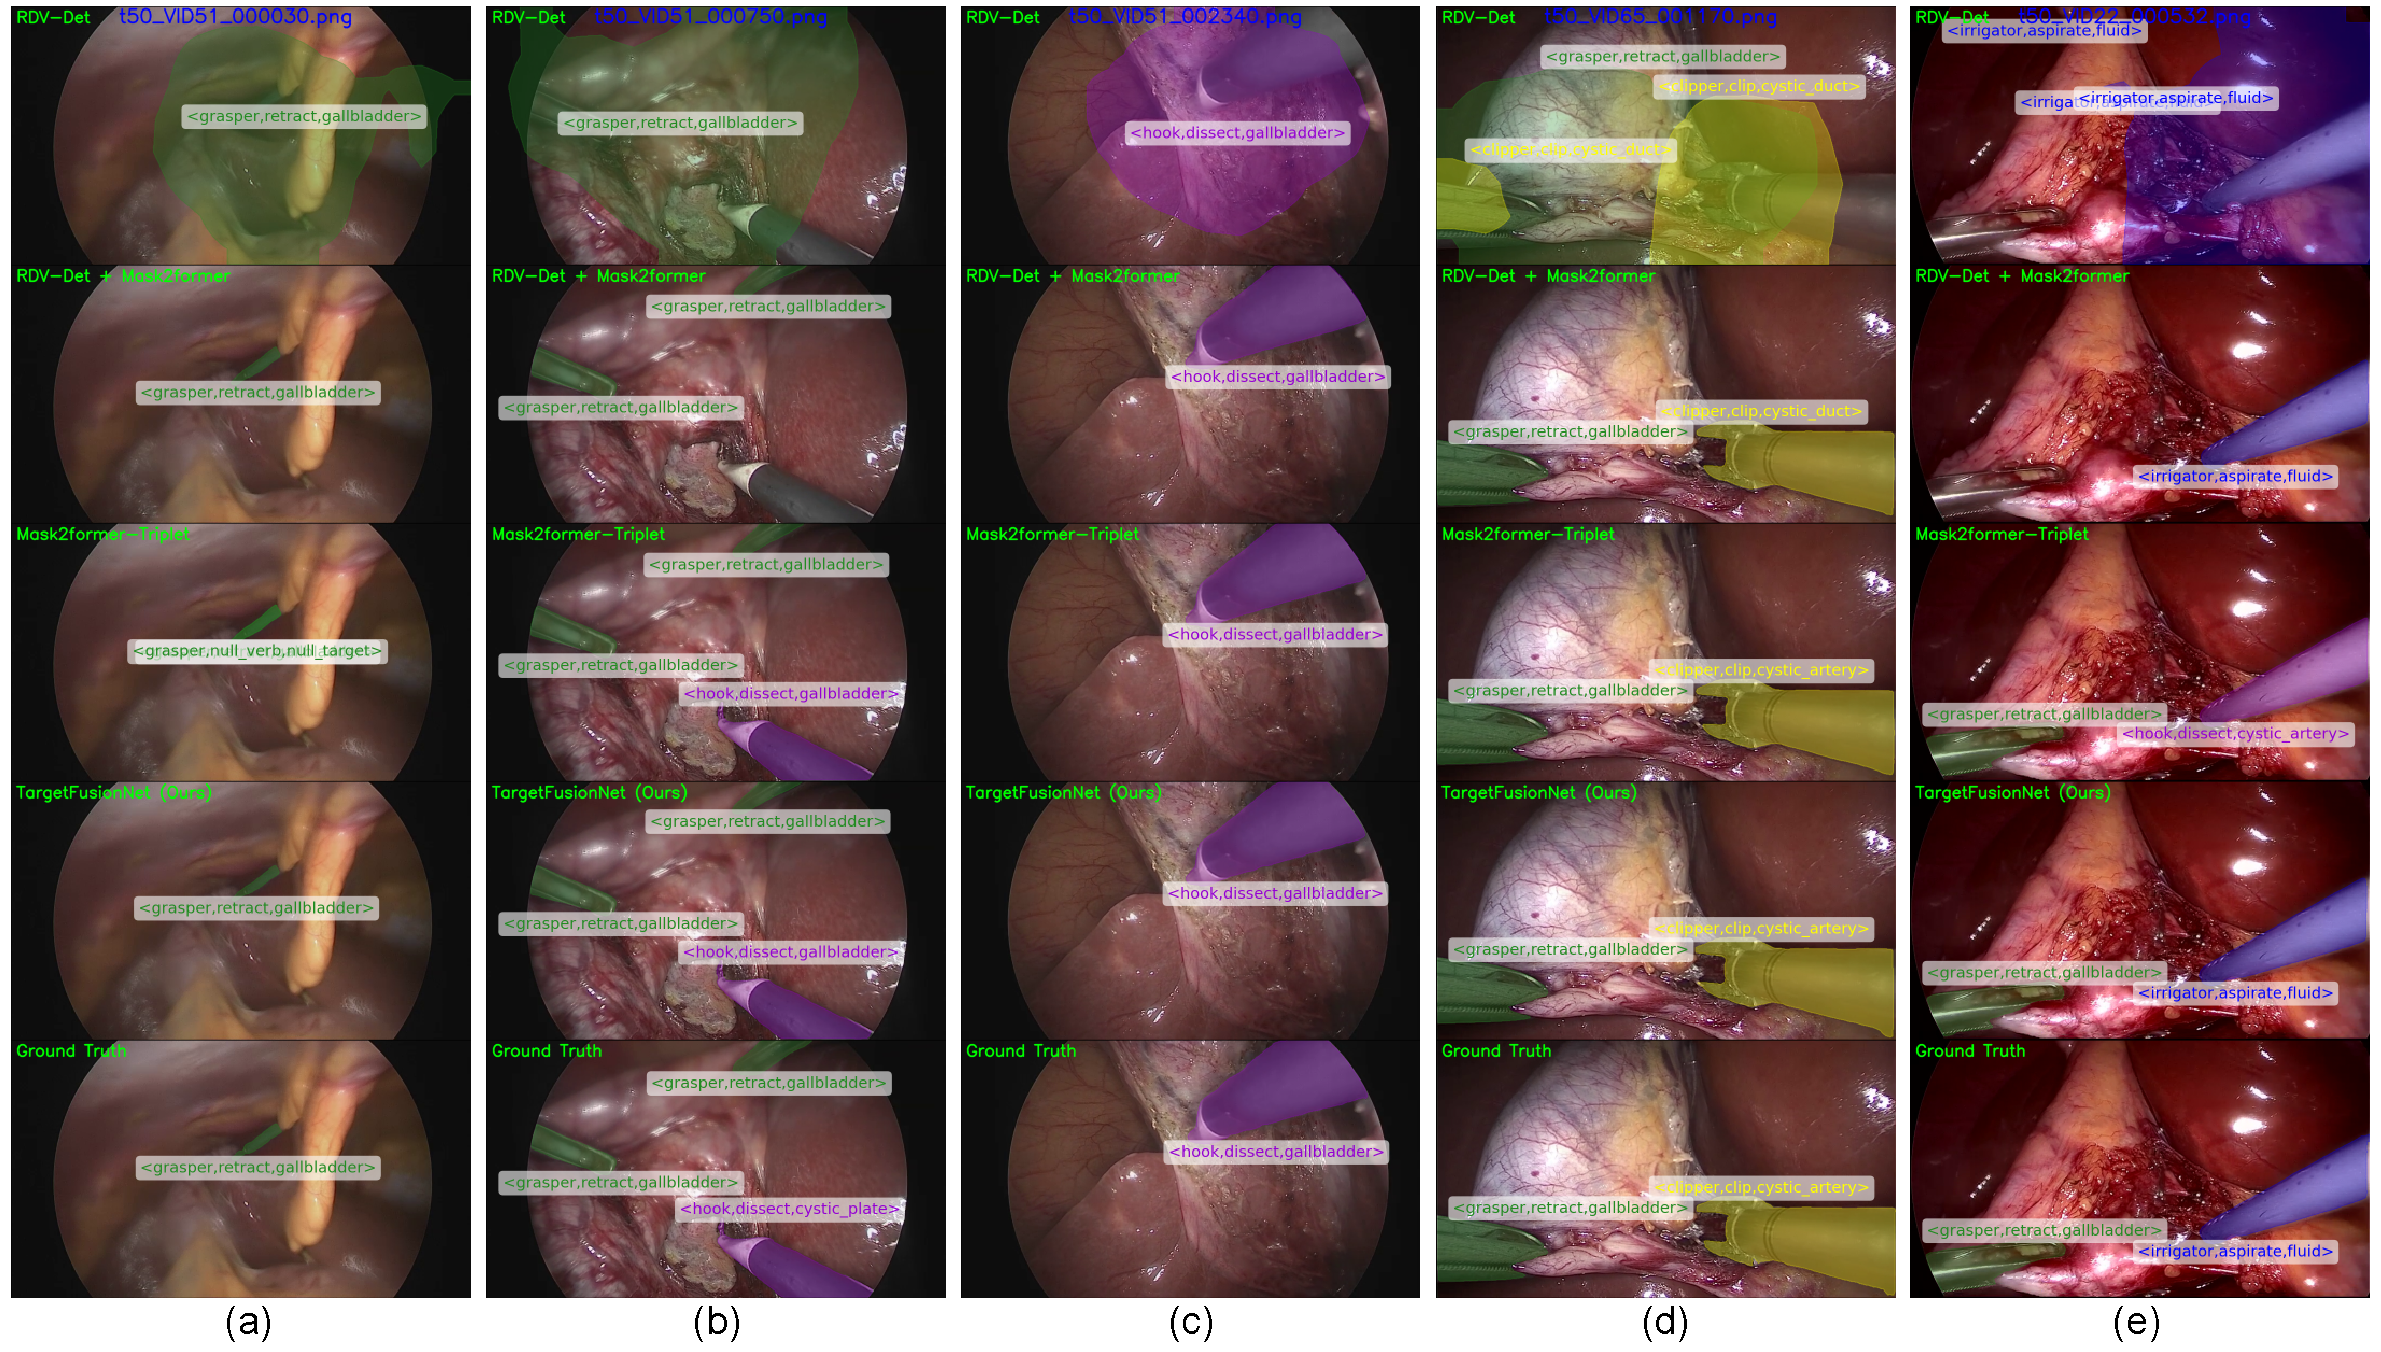
\includegraphics[width=\linewidth]{figs/triplet_grounding/qualitative.pdf}
\caption{Qualitative comparison of grounded triplet predictions. TargetFusionNet improves spatial grounding and triplet consistency in complex multi-instrument scenes.}
\label{fig:triplet-grounding-qualitative}
\end{figure}

\section{Failure Modes and Limitations}
\label{sec:triplet-grounding-limitations}

Despite the improvements from strong instance supervision and target-aware fusion, triplet segmentation remains difficult. The most important limitation is target prediction. Anatomical targets can be visually similar, weakly bounded, partially occluded, or defined by surgical context rather than appearance alone. This is why target mAP remains much lower than instrument mAP across all methods.

\begin{figure}[ht]
\centering
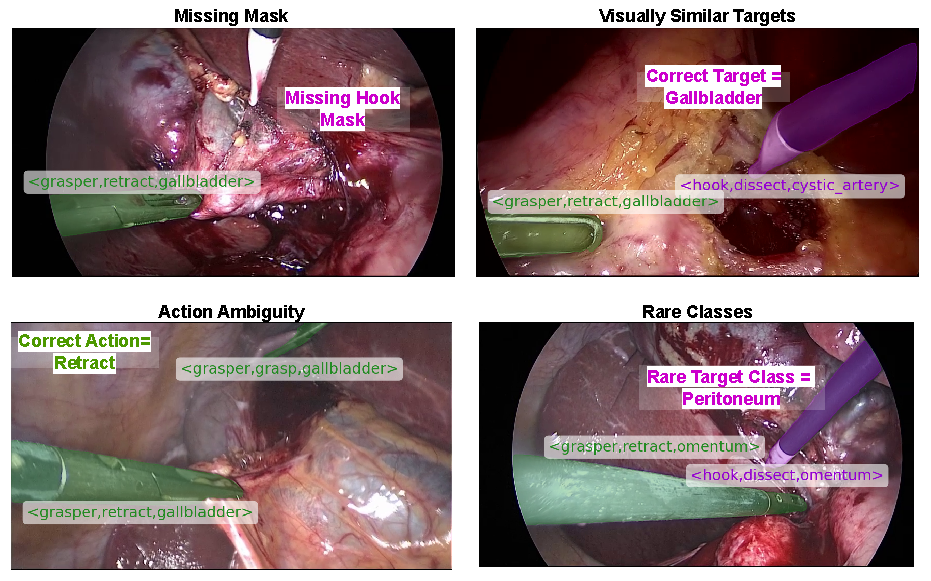
\includegraphics[width=\linewidth]{figs/triplet_grounding/failure_modes.pdf}
\caption{Representative triplet segmentation failure modes, including missing masks, confusion between visually similar anatomical targets, verb ambiguity, and errors on rare target classes.}
\label{fig:triplet-grounding-failure-modes}
\end{figure}

Four recurring failure modes were observed. First, missing or incorrect instrument masks can cause the entire triplet prediction to fail, since triplet segmentation depends on accurate instance localisation. Second, rare triplet classes are difficult to learn because they have limited supervision. Third, visually similar targets such as cystic duct, cystic artery, cystic pedicle, and gallbladder are often confused. Fourth, some verbs are difficult to distinguish in single frames; for example, grasping and retracting may look similar without temporal context.

The long-tailed distribution of triplets further amplifies these issues. When triplet classes are grouped by frequency, performance decreases sharply for rare classes.

\begin{table}[ht]
\centering
\begin{tabular}{l|c|c|c}
\hline
\textbf{Triplet group} & \textbf{Classes} & \textbf{Avg. samples/class} & \(\tripmap_{IVT}^{seg}\) \\
\hline
Frequent & 10 & 4168.9 & 0.4148 \\
Medium-frequency & 21 & 307.9 & 0.2071 \\
Rare & 62 & 24.9 & 0.04 \\
\hline
\end{tabular}
\caption{Triplet segmentation performance grouped by training frequency. Rare triplets are substantially harder to predict.}
\label{tab:triplet-grounding-frequency-analysis}
\end{table}

These limitations motivate the next chapter. TargetFusionNet treats anatomical information as a weak visual prior and fuses it into a representation-learning model. However, many target errors appear to require reasoning about anatomical context, instrument position, and surgical intent. \Chapref{chap:target-reasoning} therefore explores whether target prediction should be approached not only as a feature-fusion problem, but also as a reasoning problem.

\section{Conclusion}
\label{sec:triplet-grounding-conclusion}

This chapter introduced triplet segmentation as a spatially grounded formulation of surgical action triplet understanding. By aligning CholecT50 triplet labels with CholecInstanceSeg instrument masks, CholecTriplet-Seg provides the first benchmark in this thesis for instance-level grounding of instrument-verb-target interactions. TargetFusionNet improves over weakly grounded and strongly supervised baselines by incorporating weak anatomical priors through gated decoder-level fusion.

The results show that strong instrument instance supervision is essential for grounded surgical interaction understanding, but also that target prediction remains the main bottleneck. This observation provides the conceptual bridge to the next chapter, which investigates target prediction through explicit reasoning with vision-language models.
